%!TEX root=paper.tex

\section{Identity-Based Grouping of Requests}
\label{sec:grouping}

It is sometimes the case that the utilization and performance of an API must be understood not only per endpoint, but also by grouping the requests by another criterion. Two such examples are: 
\begin{itemize}
	\item When a service has diferent types of users (e.g. the paying vs. the free-for-evaluation ones, or the in-house vs. those in a different organization) the maintainer must understand the performance for the different groups
	\item When the load mix of the users can vary dramatically and the system response time is a function of the individual user load\footnote{E.g. in GMail some users have a few dozen emails while other have tens of thousands: this difference in user loads will eventually induce a difference in the response times for different users} the maintainer must understand the variation of performance with the users (and implicitly the user load).
\end{itemize}

To support narrowing down the analysis to groups of users, or even individual users, the \tool can log together with every request grouping information for that request. The simplest way of achieving this is to take advantage of the architecture of Flask applications in which a global \code{flask.request} is used to retrieve session information which can in turn is normally used to identify the user sending the request. From the user one can obtain the group. 

%\niceseparator

The following code snippet shows how we enabled \tool to enable user-by-user analysis\footnote{If we wanted to group by the user group for example, the code would change slightly by replacing ``user.id'' with ``user.group.id''}: 

\begin{lstlisting}[style=custompython]  
# LOC #2: configure the dashboard
# to group requests by the user id
dashboard.config.group_by = 'User',
  lambda: Session.find(flask.request).user.id

\end{lstlisting}

The \code{dashboard.config.group\_by} is assigned a tuple with two elements, in which:  

\begin{itemize}
	\item \code{'User'} stands for the name of this particular grouping strategy
	\item \code{lambda: Session.find... } is a callback with no arguments, 
	that makes use of the global \code{flask.request} and extracts from 
	the request the current session, and in turn the user id\footnote{
		Note that every web service or application must have a way of 
		associating a request with a user. In fact, the Session.find(request) 
		was already an existing function in the analyzed system}
\end{itemize}


In Zeeguu, it was decided to further understand the per-user performance of \epFeedItems
~---  an endpoint that retrieves a list of recommended articles for a given user.
It is the endpoint with the slowest response time and highest variability (see \Fref{fig:ep}). 


\begin{figure}[h!]
  \centering
  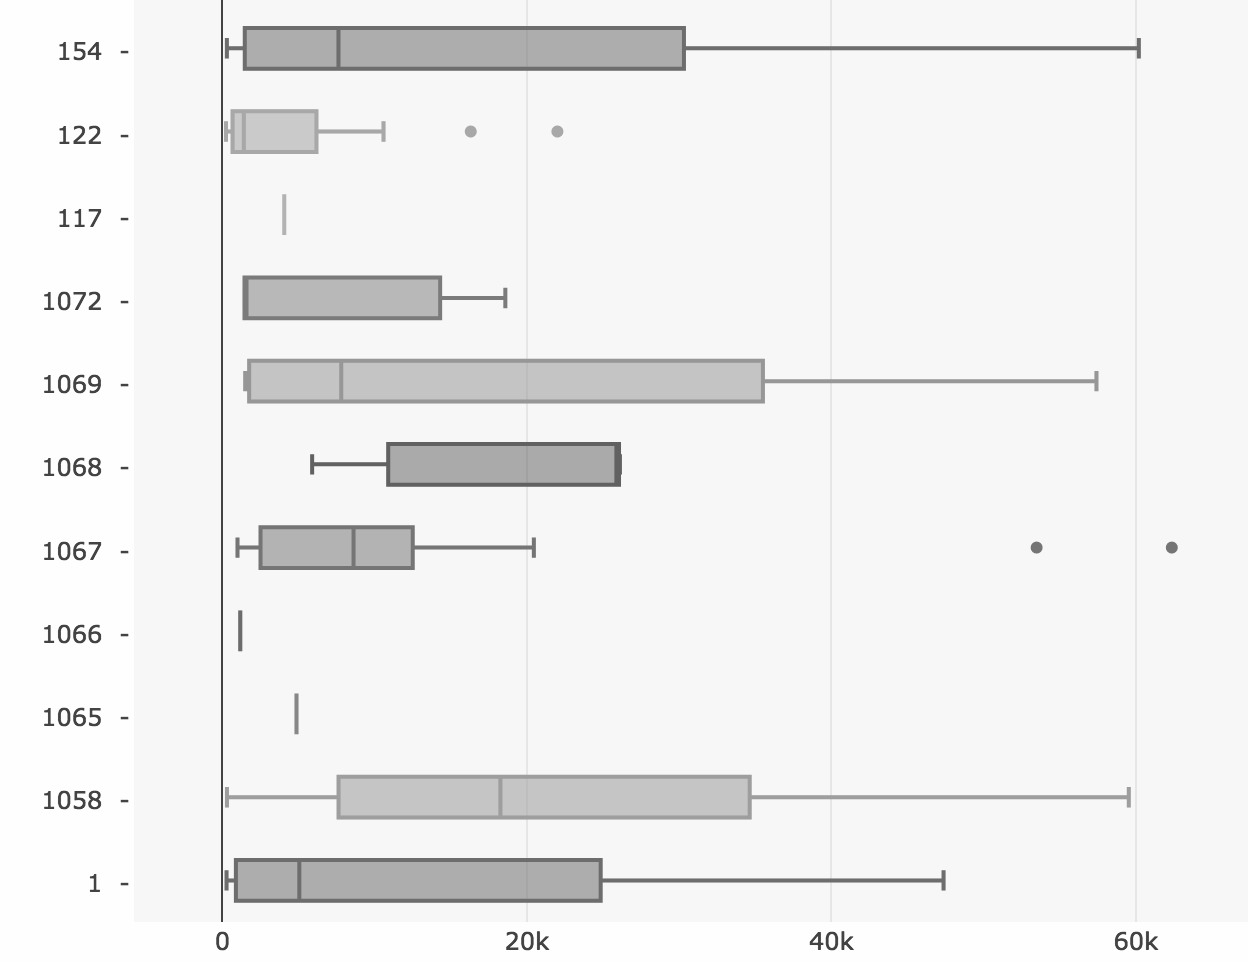
\includegraphics[width=.7\linewidth]{time_per_user}
  \caption{The \epFeedItems shows a very high variability across users}
  \label{fig:tpu}
\end{figure}


After configuring the \tool as shown earlier, the \perspective{Per-User Endpoint Performance} perspective becomes available to  present the different response times for different users. Figure \ref{fig:tpu} presents a subset of the corresponding view in the \tool. The figure shows that the response times for this endpoint varied considerably for different users with some extreme cases where a user has to wait a full minute until their recommended articles were shown. 

The reason for this behavior is that a user can be subscribed to anything from one to three dozen 
article sources and for each of the sources the system computed the personalized difficulty 
of each article at every request. After seeing the two perspectives presented in Figures \ref{fig:ep} and \ref{fig:tpu}, the \zee maintainer refactored the architecture of the system to move this difficult computation out of the interactive loop.






